%Chapter 3

\renewcommand{\thechapter}{3}

\chapter{Spin-Orbit coupling and Anderson localization in a cold-atom system}
In contrast to a condensed-matter system where we have little control over the material structure and the internal environment of particles, in a cold-atoms system, the external potential, the coupling between internal states and the interaction between particles can all be artificially engineered in the lab. Using the interaction between atoms and the electromagnetic field, the Hamiltonian of the atoms can be engineered to simulate that of particles in a condensed-matter system. The parameters in the Hamiltonian can be tuned by changing the intensity of the light, frequency of the light, the strength of the electromagnetic field, and etc. The high level of control over a cold-atoms system and the ability to simulate the Hamiltonian of a condensed-matter system make it an ideal platform to study fundamental condensed-matter physics that is otherwise hard to study. 

Spin-orbit coupling and Anderson localization have been realized and studied in cold atoms over the last decade. In this chapter, we briefly review the progress of spin-orbit coupling and Anderson localization in cold atoms on which our research of spin-orbit coupling enhanced transport in a random field is based.

\section{Spin-orbit coupling}



\subsection{Origin of SOC in a solid-state system}
a
\newpage
\section{Anderson Localization}

Anderson Localization (AL), introduced in 1958~\cite{anderson1958absence}, describes the localization of quantum waves in disordered media. Anderson studied the evolution of a wave packet undergoing multiple scattering processes from a random potential and proved the scattered waves can constructively interfere, leading to localization. This general starting point makes AL applicable to many quantum systems including: optical waves in disordered media~\cite{wiersma1997localization,scheffold1999localization,storzer2006observation}, electrons imperfect in crystals~\cite{anderson1958absence} and matter waves in disordered optical potentials~\cite{sanchez2007anderson,billy2008direct,roati2008anderson,kondov2011three}.

After AL was observed in multiple systems, in recent years, the research topic of AL phase transition in many body systems (may body localization) has attracted more attentions \cite{pal2010many,bardarson2012unbounded,schreiber2015observation,nandkishore2015many,choi2016exploring}. When disorder strength is above a critical value, the many body system undergoes a phase transition from thermalizing ergodic phase to a nonergodic phase. And in the nonergodic phase, the initial ordering of the many body system persists, which leads to potential application in quantum information \cite{schreiber2015observation,nandkishore2015many}. 

In this section, we first introduce a simple model from \cite{anderson1958absence} that catches the basic idea of single particle AL. Next, we review the progress of AL in cold atoms.
\subsection{Introduction to Anderson Localization}
% \begin{figure}[htbp]
%     \centering
%     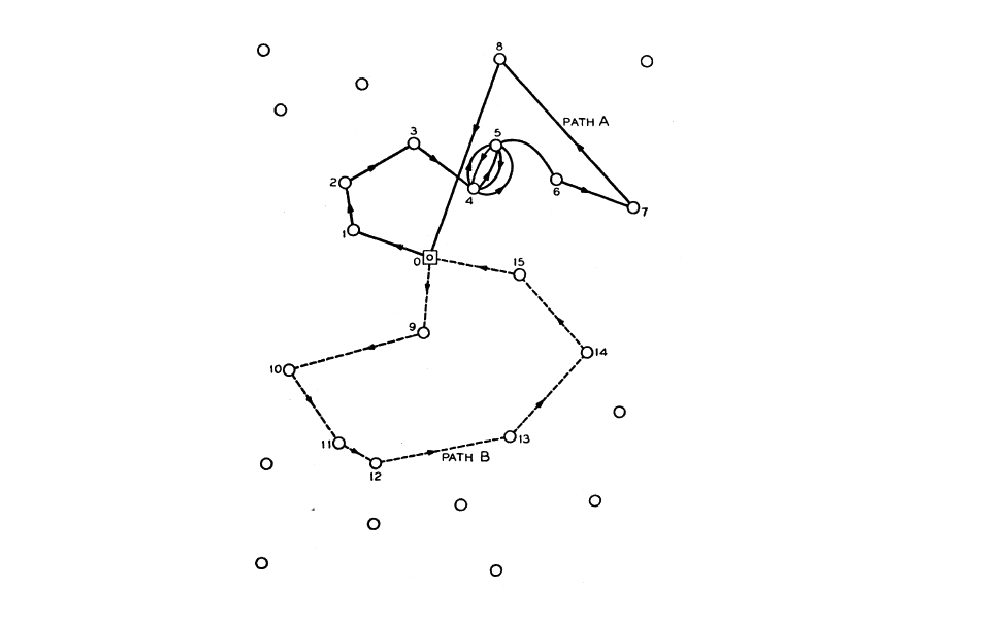
\includegraphics[width=\textwidth]{Chapter3_secs/AL1.pdf}
%     \caption{Fig.~(1) in \cite{anderson1958absence}, two kinds of scattering paths originated from lattice site 0. Path A may be large and must be summed over. Path B is a legitimate term. The potential energy at each lattice site j, $E_j$ is a random variable.}
%     \label{fig:AL1}
% \end{figure}

In the paper that introduced AL \cite{anderson1958absence}, the author studied the motion of some mobile entities in certain random lattices. It can be spins in a random field or electrons in a disordered crystal. The entities move by jumping from site to site. Starting from the most general case, the wave function of an entity can be expanded in the basis of the Wannier functions on each lattice site, 
\begin{equation}
    \hat{\psi}(\Vec{r}) = \sum_j W(\Vec{r}-\Vec{r}_j)\hat{a}_j.
\end{equation}
The Hamiltonian is
\begin{equation}
    \hat{H} = \sum_j E_j \hat{a}_j^\dag\hat{a}_j + \sum_{j<k}(V_{jk}\hat{a}_j^\dag\hat{a}_k + c.c)
\end{equation}
Here $E_j$ is the potential energy at site $j$, it is a random variable and has probability density distribution $E_j \sim \mathbb{P}(E)dE$ which is characterized by a width $W$. $V_{jk}$ is the coupling of states on site $j$ and site $k$, it can be random or non-random.

Under the following two conditions, it was proved in \cite{anderson1958absence} the wave function will be localized in a small region without diffusion. Here localization means at $t=0$, starting at site $j$, $a_j(0) = 1$, and $a_j(\infty)$ remains finite.
\begin{itemize}
    \item Low density of sites. The average coupling strength between states at different lattice sites $\langle V_{jk} \rangle < V_c$, $V_c$ is of the magnitude of $W$.
    \item $V(r)$ falls off faster than $\frac{1}{r^3}$ as $r \to \infty$.
\end{itemize}

Intuitively, the probability of diffusion from the initial site $j$ depends on the number of energy matching sites $k$ and the coupling strength between site $j$ and sites $k$. Starting from the original state at site $j$, consider the sites $k$ within the sphere of radius $r$ originated from the site $j$. As $r$ increases, the probability of finding more energy matching sites $k$ within the sphere of radius $r$ increases as $r^3$ in a 3-dimensional space. But if the coupling strength $V(r)$ decreases even faster, as $r \to \infty$, the probability the initial state diffuses to other sites remains small. So under the two conditions above, no diffusion happens and the initial state is localized.

The following discussion in \cite{anderson1958absence} shows in theory how diffusion happens. Laplace transform $a_j(t)$, the probability amplitude at site $j$,
\begin{equation}
    f_j(s) = \int^\infty_0e^{-st}a_j(t)dt
\end{equation}
Schr\"{o}dinger's equation is
\begin{equation}
    i[sf_j(s)-a_j(0)] = E_jf_j + \sum_{k\neq j}V_{jk}f_k
\end{equation}
By evaluating 
\begin{equation}
    \lim_{s \to 0^+}sf_j(s)  = a_j(0)
\end{equation}
the condition of localization can be studied. The following two infinite series describe how $f_j(s)$ evolves.
\begin{align}
    &f_0(s) - \frac{i}{is-E_0} + \sum_k \frac{1}{is-E_0}V_{0k}\left(\frac{V_{0k}}{is-E_k} + \sum_l\frac{1}{is-E_l}V_{kl}\frac{1}{is-E_k}V_{l0} + \cdots \right)f_0(s)\\\nonumber
    &f_j(s) = \frac{1}{is-E_j}V_{j0}f_0(s) + \sum_k\frac{i}{is-E_j}V_{jk}\frac{i}{is-E_k}f_0(s) + \cdots\\\nonumber
\end{align}
The infinite series describe the high-order scattering processes, diffusion happens if the initial state goes through different scattering paths that constructively interfere at other sites.  
The term 
\begin{equation}
    V_c(s) = \sum_k \frac{V_{0k}^2}{is-E_k} + \sum_{k,l}
    \frac{V_{0k}V_{kl}V_{l0}}{(is-E_k)(is-E_l)} + \cdots
\end{equation}
describes the strength of diffusion through infinite orders of scattering. By considering only the direct connections between the initial site and the neighbors, the second-order approximation is made. 
\begin{equation}
    f_0(s) = \frac{i}{is(1+K) + (i/\tau) - (E_0 - \Delta E^{(2)})}
\end{equation}
Here, 
\begin{align}
    &1/\tau = \sum_kV_{0k}^2\delta(E_k)\\\nonumber
    &K = \sum_{E_k\neq 0}\frac{V_{0k}^2}{E_k^{(2)}}
\end{align}
and $E^{(2)}$ is the second-order energy perturbation. When $\tau$ is finite, meaning there are some energy matching sites coupled to the initial site, the amplitude $a_0(t)$ decays at $e^{-t/\tau}$, and the diffusion happens. Otherwise, when no energy matching states are coupled to the initial site, the amplitude does not decay, instead, it spreads by the ratio $1/(1+K)$. No real transport happens in this case, the initial state is localized.

\subsection{AL in cold atoms}
AL was originally introduced in a condensed matter system, for example, electrons in a disordered crystal and spins in a disordered field. But there are a number of difficulties for observing AL in a condensed matter system. The interaction between electrons is hard to change, there are no good methods to directly measure the wave function of electrons in a solid. In contrast, cold atoms is an ideal platform to study AL. The interaction bwtween atoms can be tuned negligible, the wave function of atoms can be directly measured by absorption imaging and optical dipole potential has been developed that enables optical lattices.

1D AL was first observed in cold atoms in 2008 \cite{billy2008direct,roati2008anderson}. In both the experiments, the disordered potential was realized with optical dipole potential. In \cite{billy2008direct}, optical speckle from far blue detuned light was used. The statistical properties of optical speckle was well studied in the 1970s \cite{goodman2007speckle}. In \cite{roati2008anderson}, one-dimensional optical lattice perturbed by a second, weak incommensurate lattice yields localization effect. And the dependence of localization on disordered strength was studied. Later in 2011, 3D Al was realized \cite{kondov2011three}. The researchers observed three-dimensional AL of noninteracting ultracold matter by allowing a spin-polarized atomic Fermi gas to expand into a disordered
potential. In this experiment, mobility edge was extracted. In lower dimensions, actual mobility edge does not exist but quasi-mobility edge as a function of the correlation length of disordered potential has significant effect on the spread of wave function \cite{sanchez2007anderson,billy2008direct}.

\begin{figure}[htbp]
    \centering
    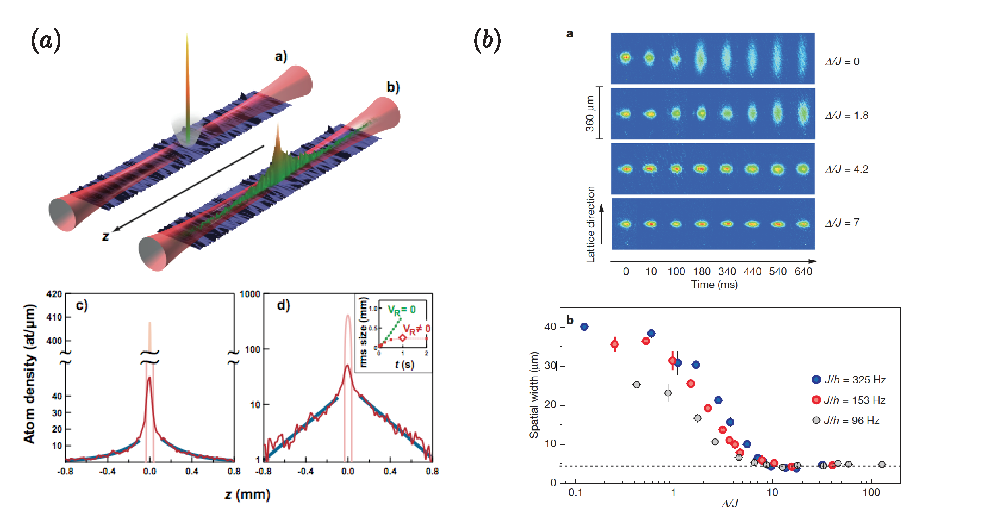
\includegraphics[width=\textwidth]{Chapter3_secs/AL2.pdf}
    \caption{First 1D AL experiments in cold atoms. (a). Fig.~(1) in \cite{billy2008direct}, Observation of exponential localization. (b). Fig.~(2) in \cite{roati2008anderson}, Probing the localization with transport. }
    \label{fig:AL2}
\end{figure}

As shown in Fig.~(\ref{fig:AL2})(a), a BEC is made in a hybrid trap consisting of a dipole trap and a magnetic trap providing longitudinal confinement. 1d optical speckle along the dipole trap was added. At t=0, the magnetic trap was turned off and the BEC started expanding due to the repulsive interaction. Without the optical speckle, the width of the atoms grow linearly in time, and as they expand, the density drops and the interaction becomes negligible. In this process, the interaction is converted into kinetic energy and determines $k_{max}$ in the momentum distribution. It is predicted in theory \cite{sanchez2007anderson} for a speckle potential with intensity correlation length $\sigma_R$, when $k_{max}\sigma_R<1$, the localized wave function has a tail that exponentially decays. This is a feature of AL. When $k_{max}\sigma_R>1$, the density profiles should have algebraic wings. $\sigma_R$ determine the quasi-mobility edge in 1D.

In Fig.~(\ref{fig:AL2})(b), 1D AL was observed in one-dimensional quasi-periodic lattice. The system is described by a Anbry-Andr\'{e} model \cite{aubry1980analyticity,harper1955single}
\begin{equation}
    \hat{H} = J\sum_m (\dyad{w_m}{w_{m+1}} + \dyad{w_m}{w_{m+1}}) + \Delta\sum_m \cos{2\pi\beta m + \phi}\dyad{w_m}{w_m}.
\end{equation}
$\ket{w_m}$ is the Wannier function at lattice m, $J$ is the tunnelling energy and $\Delta$ is the strength of disorder. The researcher make the noninteracting BEC expand along the 1D lattice, and measure the spatial density as a function of time and disorder strength. As  the disorder strength $\Delta/J$ goes above a critical value, they observed a crossover between ballistic expansion of BEC and no expansion. They demonstrated the system has the feature as in the case of purely random disorder in higher dimensions. 

These research works paved the way for more sophisticated AL studies in cold atoms and enables the interplay between AL and other well studied topics in cold atoms, for example, spin-orbit coupling.




